\documentclass[12pt]{article}
\usepackage{amsfonts, amssymb, amsthm}
\usepackage{amsmath}
\usepackage{tikz}

\pagestyle{myheadings}
\markright{Simon Kurgan\hfill\today\hfill}

\newtheorem{theorem}{Theorem}[section]
\newtheorem{corollary}{Corollary}[theorem]

\begin{document}

\section{Introduction}

\begin{theorem}
    A sequence is an infinite list of numbers that are indexed by $\mathbb{N}$ or a subset of $\mathbb{N}$. We can often write a sequence in the form $a_1, a_2, ... a_n$
\end{theorem}

\begin{proof}[Example:]
    $(A_n)_{n=0}^\infty$
\end{proof}

\begin{theorem}
    We can define a sequence recursively (recursive definition). The Fibonacci sequence $f_n$ is defined as follows:
\end{theorem}

\begin{proof}[Example:]
    \[
    f_n = 
        \begin{cases}
        f_0 = 1, f_1 = 1 \\
        f_{n+2} = f_{n+1} + f_n \text{ if } n \geq 0.
        \end{cases}
    \]
\end{proof}

\newpage

\begin{theorem}
    For each $n \in \mathbb{N}$, the Fibonacci number $f_{3n}$ is an even natural number.
\end{theorem}

\begin{proof}[Proof:]
    We prove this by induction.

    Base case: when $n = 0, f_0$ is even.

    Inductive step: Suppose $f_{3k}$ is even for some $k \geq 0$

    We want to prove $f_{3(k+1)}$ is even

    Note $f_{3(k+1)}$ = $f_{3k+3}$

    By the recursive definition, $f_{3k+3}$ = $f_{3k+2}$ + $f_{3k+1}$

    Further simplifying, ($f_{3k+1}$ + $f_{3k}$) + $f_{3k+1}$

    $2f_{3k+1} + f_{3k}$

    Substituting, $2f_{3k+1} + 2L$

    Thus, $2(f_{3k+1} + L)$ is even.

    By the closure of the set of integers and the recursive definition, this is an integer.

    By induction, this statement is true for any $\mathbb{N}$ 
\end{proof}

\newpage

\begin{theorem}
    How many ways can you tile a 2 by n grid with dominoes?
\end{theorem}

\begin{proof}[Illustrated:]

    Working from a simpler case, suppose n = 1. There is only one way to fill the grid.

    When n = 2, there are only two ways like such $\|$ and $=$

    When n = 3, there are 3 ways in which you can tile the dominoes

    When n = 4, there are 5 ways.

    When n = 5, there are 8 ways.
\end{proof}

\begin{proof}[Illustrated:]
    For any integer $n \geq 1$, the number of ways to tile a 2 by n grid with dominoes is the (n+1)th Fibonacci number, $f_{n+1}$

    Recall,

    \[
    f_n = 
        \begin{cases}
        f_0 = 1, f_1 = 1 \\
        f_{n+2} = f_{n+1} + f_n \text{ if } n \geq 0.
        \end{cases}
    \]

    Proof using induction.

    Base Case: 
    
    Suppose n = 1. There is 1 way to tile a 2 by 1 grid and $f_1 = 1$

    Suppose n = 2. There are 2 ways to tile a 2 by 2 grid and $f_3 = 2$

    Inductive Case: 
    
    Suppose the number of ways to tile an n by k grid is $f_{k + 1}$

    Suppose the number of ways to tile a 2 by (k + 1) grid is $f_{k + 2}$

    Goal: Find out the number of ways to tile a 2 by (k + 2) grid.

    Consider the top left square of this 2 by (k + 2) grid.

    There are only two ways in which it can be covered

    Case 1: 

    This square is covered by a vertical d.

    The remaining part is a 2 by (k + 1) grid.

    By the inductive hypothesis, there are $f_{k + 2}$ to cover the grid.

    Case 2:

    The square is covered by a horizontal d.

    The square underneath it must be covered by a horizontal domino.

    The remaining grid is a 2 by k grid. Which has $f_{k + 1}$ ways to tile.
\end{proof}

\newpage


Technique: Strong Mathematical Induction.


Base case: Prove $P(K_{0})$ is true

Inductive Step: For every integer $k \geq k_0$, prove P(k + 1) is true under the assumption that it is true for all smaller cases, instead of assuming that it is true for one case. 

Thus we are proving $P(K_0) \land P(K_0 + 1)$ ... $\land P(k) \implies P(k + 1)$

\begin{proof}[Theorem:] 
    Every positive integer $n \geq 2$ is either a prime number or is a product of prime numbers.
\end{proof}

\newpage

Let X, Y be two sets. The union of X and Y, denoted by $X \cup Y$ is $\{ x \in U | x \in X $ or $ x \in Y \}$

The intersection of X and Y, denote by $X \cap Y$, is $\{ x \in U | x \in X $ and $ x \in Y \}$

The set difference of X and Y (relative complement of Y w.r.t X), denoted by $X - Y$ (or $X \backslash Y$) is $\{ x \in U | x \in Y $ and $ x \notin X \}$

\medbreak

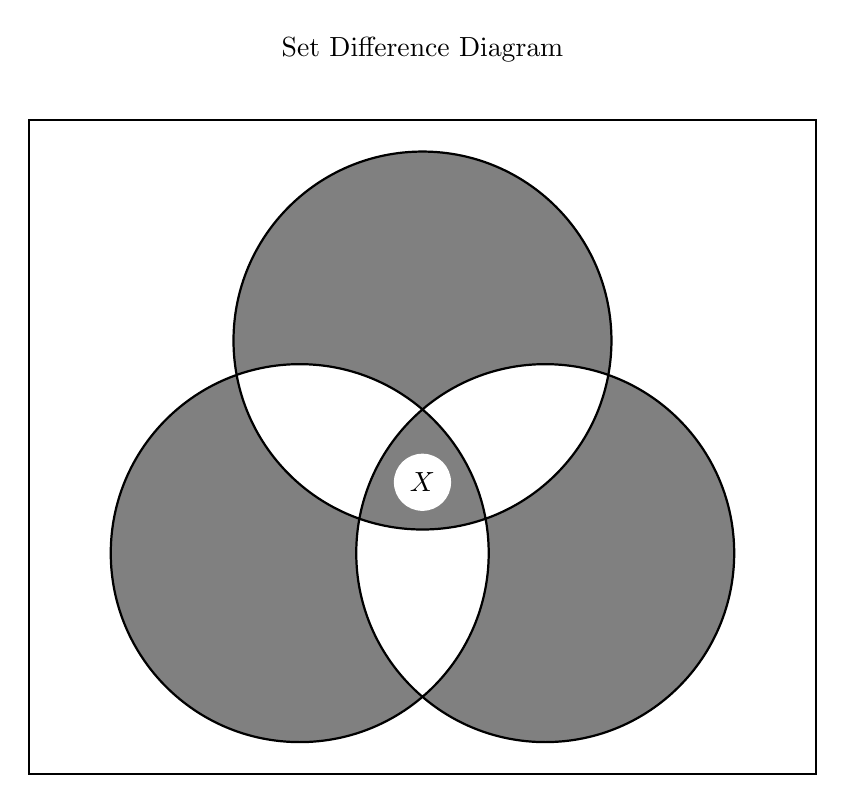
\begin{tikzpicture}
    \def\firstcircle{(90:1.8) circle[radius = 2.4]}
    \def\secondcircle{(210:1.8) circle[radius = 2.4]}
    \def\thirdcircle{(330:1.8) circle[radius = 2.4]}
  
    \draw (0, 5.5) node {Set Difference Diagram};
    \draw[thick] (-5, -3.7) rectangle (5, 4.6);
  
    \fill[even odd rule, gray] \firstcircle \secondcircle \thirdcircle;
    \draw[thick] \firstcircle \secondcircle \thirdcircle;
  
    \node[fill = white, shape = circle] (0,0) {$X$};
\end{tikzpicture}

\medbreak

The complement of $X^c$ is regarded as $U - X$ (The universal set minus the set X)

\medbreak

\textbf{Example Problem: }

Let X = $\{1, 2, 3, 4\}$

Let Y = $\{ x \in \mathbb{R} | -1 < x \leq 3 \}$

$X \cup Y$  = 1, 2, 3, 4

$X \cap Y$ = 0, 1, 2, 3

$X \backslash Y$ = 4

$Y \backslash X$ = 0

$Y^c$ = $\{ x \in \mathbb{U} | x \leq -1 $ or $ x \geq 3 \}$

\newpage

\textbf{Power Set:} Let $U$ be the universal set and let $A$ be a subset of $U$. The power set of $A$, denoted by $\mathcal{P}(A)$, is the set of all subsets of $A$, that is $\mathcal{P}(A) = \{Y \subseteq U \mid Y \subseteq A\}$.

\smallbreak

\textbf{Example 1:}

Let $U = \mathbb{R}$ and $A = \{1, 2\}$.

Subsets of $A$: $\emptyset$, $\{1\}$, $\{2\}$, $\{1, 2\}$.

$\mathcal{P}(A) = \{\emptyset, \{1\}, \{2\}, \{1, 2\}\}$.

\smallbreak

\textbf{Example 2:}

Let $U = \mathbb{R}$ and $A = \{-1, 4, 7\}$.

Subsets of $A$: $\emptyset$, $\{-1\}$, $\{4\}$, $\{7\}$, $\{-1, 4\}$, $\{-1, 7\}$, $\{4, 7\}$, $\{-1, 4, 7\}$.

$\mathcal{P}(A) = \{\emptyset, \{-1\}, \{4\}, \{7\}, \{-1, 4\}, \{-1, 7\}, \{4, 7\}, \{-1, 4, 7\}\}$.

\medbreak

\textbf{Cardinality: }

The cardinality of a finite set is the number of elements of the set.

Card(A), where $A = \{-1, 4, 7\}$ is equal to 3. 

\textbf{Question: }

Suppose $\text{card}(A) = n$. What is $\text{card}(\mathcal{P}(A))$?

\[
\text{card}(\mathcal{P}(A)) = 2^n
\]

\medbreak

\textbf{Theorem: } If A is a finite set with $\text{card}(A) = n$, then $\text{card}(\mathcal{P}(A)) = 2^n$

\begin{proof}[Proof:]
    We prove it by induction.

    \textbf{(1) Base Case:} $n = 0$, so $A = \emptyset$. 
    \[ \mathcal{P}(A) = \{\emptyset\} \]
    Therefore, 
    \[ \text{card}(\mathcal{P}(A)) = 1 = 2^0 \]
    
    \textbf{(2) Inductive Step:} Suppose any finite set $A$ with $\text{card}(A) = k$ has a power set $\mathcal{P}(A)$ with cardinality $2^k$.

    Now consider a set with card = $k + 1$.

    Here we focus on the $(k + 1)th$ element, $A_{k + 1}$

    For any subset of A, we only have 2 possiblities.

    Case 1: This subset contains $A_{k + 1}$. If we remove $A_{k + 1}$ from this subset, we get a subset of a set with card $= k$.

    By the inductive hypothesis, we have $2^k$ possiblities for such subsets.

    Case 2: This subset does not contain $A_{k + 1}$. Then it is a subset of a set with card $= k$. By the inductive hypothesis, we have $2^k$ in this case. Thus, A has $2^k + 2^k = 2^{k+1}$ possibilities of subsets.
\end{proof}

\medbreak

\textbf{Technique (Element Chasing): }

To prove $A \subseteq B$, for every $x \in A$, prove $x \in B$.

To disprove $A \subseteq B$, give an example of some $x \in A$ such that $x \notin B$.

\medbreak

\begin{theorem}
    Suppose $A, B, C$ are subsets. Then $A \setminus (B \cup C) \subseteq (A \setminus B) \cup (A \setminus C)$.
\end{theorem}

\begin{proof}[Proof:]
    Let $x \in A \setminus (B \cup C)$, which means $x \in A$ and $x \notin (B \cup C)$.

    Since $x \in A$ and $x \notin B$, then $x \in A \setminus B$.

    Then by the definition of the union of two sets, $x \in (A \setminus B) \cup (A \setminus C)$.

    We conclude $A \setminus (B \cup C) \subseteq (A \setminus B) \cup (A \setminus C)$.
\end{proof}

\textbf{Question: } Do we have $(A \setminus B) \cup (A \setminus C) \subseteq A \setminus (B \cup C)$?

Counterexample:

$A = \{1, 2, 3\}$

$B = \{2\}$

$C = \{3\}$

$A \setminus B = \{1, 3\}$

$A \setminus C = \{1, 2\}$

$(A \setminus B) \cup (A \setminus C) = \{1, 2, 3\}$

\begin{theorem}
    Suppose $A, B, C$ are subsets. Then A \ (B union C) = (A \ B) intersection (A \ C)
\end{theorem}

\begin{proof}[Proof:]
    We prove two inclusions.

    (1) We prove A \ (B union C) subset (A \ B) union (A \ C)

    (2) We prove ...

\end{proof}


\end{document}
